\documentclass[11pt]{article}
\usepackage[margin=1in]{geometry}
\usepackage[T1]{fontenc}
\usepackage{lmodern}
\usepackage{microtype}
\usepackage{amsmath,amssymb,amsthm,mathtools}
\usepackage{booktabs,graphicx,xcolor,enumitem,listings}
\usepackage[colorlinks=true,linkcolor=blue!50!black,citecolor=blue!50!black,urlcolor=blue!50!black]{hyperref}

\graphicspath{{figures/}}
% generated by scripts/figs_step01.py; do not edit
\newcommand{\NCurves}{3,824,372}
\newcommand{\NClasses}{2,917,287}
\newcommand{\NSingletonClasses}{76.9\%}
\newcommand{\MaxClassSize}{8}
\newcommand{\NComplete}{3,064,705}
\newcommand{\NHigh}{759,667}
\newcommand{\NHighPrime}{727,585}
\newcommand{\NHighSmooth}{32,082}
\newcommand{\NSmallPrime}{5,525}
\newcommand{\MaxConductor}{299,996,953}
\newcommand{\NBigCoeffs}{1,228}
\newcommand{\NChecks}{10}
\newcommand{\NFailures}{0}
\newcommand{\NRankZero}{1,404,510}
\newcommand{\NRankOne}{1,887,132}
\newcommand{\NRankTwo}{493,291}
\newcommand{\NRankThree}{37,334}
\newcommand{\NRankFour}{2,086}
\newcommand{\NRankFive}{19}
\newcommand{\NTaskTwo}{1,897,801}
\newcommand{\PiTaskTwo}{26.0\%}
\newcommand{\PiTaskTwoComplete}{22.9\%}
\newcommand{\PiTaskTwoHighPrime}{39.1\%}
\newcommand{\PiTaskTwoSmallPrime}{37.0\%}
\newcommand{\RankTwoFirstBin}{5.6\%}
\newcommand{\RankTwoLastBin}{12.8\%}
\newcommand{\RankZeroFirstBin}{43.6\%}
\newcommand{\RankZeroLastBin}{37.1\%}
\newcommand{\ShaBigRankZero}{20.4\%}
\newcommand{\ShaBigRankTwo}{0.1\%}


\theoremstyle{definition}
\newtheorem{definition}{Definition}[section]
\newtheorem{exercise}{Exercise}[section]
\theoremstyle{plain}
\newtheorem{theorem}[definition]{Theorem}
\newtheorem{proposition}[definition]{Proposition}
\newtheorem{conjecture}[definition]{Conjecture}
\theoremstyle{remark}
\newtheorem{remark}[definition]{Remark}

\newcommand{\Q}{\mathbb{Q}}
\newcommand{\Z}{\mathbb{Z}}
\newcommand{\F}{\mathbb{F}}
\newcommand{\R}{\mathbb{R}}
\newcommand{\E}{\mathbb{E}}
\renewcommand{\P}{\mathbb{P}}
\newcommand{\code}[1]{\texttt{#1}}
% let long identifiers like task2\_label break after an underscore
\let\oldunderscore\_
\renewcommand{\_}{\oldunderscore\allowbreak}
\emergencystretch=1.5em
\newcommand{\file}[1]{\textcolor{blue!50!black}{\texttt{#1}}}
\DeclareMathOperator{\ord}{ord}
\DeclareMathOperator{\rk}{rk}
\DeclareMathOperator{\Sha}{Sha}
\DeclareMathOperator{\Reg}{Reg}

\definecolor{codebg}{RGB}{247,247,244}
\lstdefinestyle{py}{language=Python, basicstyle=\ttfamily\footnotesize, backgroundcolor=\color{codebg},
  keywordstyle=\color{blue!60!black}\bfseries, commentstyle=\color{green!40!black}\itshape,
  stringstyle=\color{red!50!black}, frame=l, framerule=1.5pt, rulecolor=\color{blue!40!black},
  xleftmargin=1.2em, framexleftmargin=0.6em, aboveskip=0.6em, belowskip=0.6em,
  columns=fullflexible, keepspaces=true, showstringspaces=false,
  morekeywords={match,case}}
\lstset{style=py}
% \codefrom{file}: caption line above a listing saying where it lives
\newcommand{\codefrom}[1]{\par\smallskip\noindent{\footnotesize\textbf{From} \file{#1}}}

% interview box: closes each section with how to say it out loud
\definecolor{interviewbg}{RGB}{240,245,252}
\newenvironment{interview}
  {\par\medskip\noindent\begin{lrbox}{0}\begin{minipage}{\dimexpr\linewidth-2\fboxsep-2\fboxrule\relax}
   \textbf{Interview prep.}\ }
  {\end{minipage}\end{lrbox}\fcolorbox{blue!40!black}{interviewbg}{\usebox{0}}\par\medskip}

\title{Learning the Rank of an Elliptic Curve\\[4pt]\large Lecture notes written while building \code{elliptic-curve-intelligence-lab}}
\author{Dylan Costa}
\date{}

\begin{document}
\maketitle
\tableofcontents

% Section numbers match the project's step numbers, starting at 0.
\setcounter{section}{-1}

%=============================================================================
\section{The problem: which rank are we predicting?}
\label{sec:problem}
%=============================================================================

We want a function $f$ that takes an elliptic curve $E/\Q$, given by its Weierstrass
coefficients, and returns the probability that its rank is positive (Task~1) or, among curves
of even rank, that its rank is $2$ rather than $0$ (Task~2). Computing the rank is a hard
problem with no known algorithm guaranteed to terminate. Predicting it is a statistical
question: given a few million curves whose ranks are known, which cheaply computable features of
a curve carry information about its rank, and does that information survive on curves larger
than the ones we trained on? This section pins down what ``rank'' means, which rank our labels
are, and why Task~2, not Task~1, is the honest version of the question.

\paragraph{Curves and their rational points.}
An elliptic curve over $\Q$ is a smooth projective curve given by a Weierstrass equation
\[
  E:\ y^2+a_1xy+a_3y=x^3+a_2x^2+a_4x+a_6,\qquad a_i\in\Z,
\]
with nonzero discriminant $\Delta$. Its rational points form an abelian group, and
Mordell's theorem (1922) says this group is finitely generated:
\[
  E(\Q)\ \cong\ E(\Q)_{\mathrm{tors}}\oplus\Z^{r},\qquad r=\rk E(\Q).
\]
The torsion part is well understood: by Mazur (1977) it is one of exactly 15 groups, and
it is easy to compute. The \emph{algebraic rank} $r$ is the mystery. A curve has rank
$0$ when it has only finitely many rational points, and positive rank when it has infinitely
many. Our dataset stores each curve by its label and coefficients, for example
\code{11.a1|[0,-1,1,-7820,-263580]|0|[]|11|1}: label, $[a_1,a_2,a_3,a_4,a_6]$, rank, torsion
structure, conductor, and the analytic order of the Shafarevich--Tate group $\Sha$.

\paragraph{Counting points mod $p$, and the $L$-function.}
Reducing the equation mod a prime $p$ gives a curve over $\F_p$ with some number of points.
Write
\[
  a_p\;=\;p+1-\#E(\F_p),\qquad |a_p|\le 2\sqrt p\quad\text{(Hasse, 1933) for } p\nmid N.
\]
Here $N$ is the \emph{conductor}, a product of the primes where $E$ has bad reduction
(with exponents that record how bad). The $a_p$ assemble into the $L$-function
\[
  L(E,s)=\prod_{p\nmid N}\bigl(1-a_pp^{-s}+p^{1-2s}\bigr)^{-1}\prod_{p\mid N}\bigl(1-a_pp^{-s}\bigr)^{-1},
\]
which converges for $\operatorname{Re}s>3/2$. By the modularity theorem (Wiles; Taylor--Wiles;
Breuil--Conrad--Diamond--Taylor, 2001), $L(E,s)$ extends to an entire function, and
$\Lambda(E,s)=N^{s/2}(2\pi)^{-s}\Gamma(s)L(E,s)$ satisfies the functional equation
\begin{equation}\label{eq:fe}
  \Lambda(E,s)\;=\;w\,\Lambda(E,2-s),\qquad w\in\{\pm1\}.
\end{equation}
The sign $w$ is the \emph{root number}. The \emph{analytic rank} is
$r_{\mathrm{an}}=\ord_{s=1}L(E,s)$, the order of vanishing at the center of symmetry.

\begin{conjecture}[Birch and Swinnerton-Dyer]
$r_{\mathrm{an}}=r$. Moreover the leading Taylor coefficient is
\[
  \frac{L^{(r)}(E,1)}{r!}\;=\;\frac{\Omega_E\cdot\Reg(E)\cdot\prod_{p\mid N}c_p\cdot\#\Sha(E)}{\#E(\Q)_{\mathrm{tors}}^{2}},
\]
with $\Omega_E$ the real period, $\Reg$ the regulator of a basis of $E(\Q)/\text{torsion}$,
and $c_p$ the Tamagawa numbers.
\end{conjecture}

\noindent The conjecture grew out of numerical experiments in the 1960s with exactly the
quantity we will use: Birch and Swinnerton-Dyer observed that
$\prod_{p\le X}\#E(\F_p)/p$ seems to grow like $C\,(\log X)^{r}$. Curves of higher rank have,
on average, \emph{more} points mod $p$, so their $a_p$ lean negative. That is the signal a
model can hope to find.

\paragraph{Which rank are our labels?}
For small ranks, the two ranks are known to agree, and this is what makes the labels
trustworthy.

\begin{theorem}[Gross--Zagier 1986, Kolyvagin 1989, plus modularity]
If $r_{\mathrm{an}}\le1$, then $r=r_{\mathrm{an}}$ and $\Sha(E)$ is finite.
\end{theorem}

\begin{proposition}\label{prop:labels}
Suppose $r\le3$ is proven for $E$ (by exhibiting $r$ independent points and an upper bound
from descent), that $L^{(r)}(E,1)\ne0$ has been certified numerically, and that the root
number satisfies $w=(-1)^r$. Then $r_{\mathrm{an}}=r$.
\end{proposition}

\begin{proof}
Since $L^{(r)}(E,1)\neq0$, $r_{\mathrm{an}}\le r$. If $r\le1$, then $r_{\mathrm{an}}\le1$ and the
theorem gives $r_{\mathrm{an}}=r$. If $r\ge2$, then $r_{\mathrm{an}}\le1$ is impossible, because the
theorem would force $r=r_{\mathrm{an}}\le1$. So $2\le r_{\mathrm{an}}\le r$. For $r=2$ we are done.
For $r=3$, Exercise~\ref{ex:parity} gives $w=(-1)^{r_{\mathrm{an}}}$, so $r_{\mathrm{an}}$ is odd, hence $3$.
\end{proof}

\noindent For rank $4$ the argument breaks down: $r_{\mathrm{an}}\in\{2,4\}$, and nothing known
rules out $2$. That is one reason Task~2 stops at rank~$2$. Section~1 checks how the
dataset's ranks were obtained, since the curves above conductor $500{,}000$ come from a
different source than the complete tables below it.

\paragraph{The parity shortcut, and why Task~1 is not enough.}
The root number is not a mysterious analytic quantity. It factors into local signs,
$w=-\prod_{p\mid N}w_p$, and each $w_p$ is determined by the reduction of $E$ at $p$. For
multiplicative reduction, $w_p=-a_p$, where $a_p=+1$ (split) or $-1$ (non-split). Additive
reduction is more involved but still a finite local computation. So $w$ is a cheap,
deterministic function of the coefficients, and by Exercise~\ref{ex:parity},
\[
  w=(-1)^{r_{\mathrm{an}}}.
\]
Every curve with $w=-1$ has odd, hence positive, rank. A flexible model trained on Task~1
can therefore get a large part of the way by rediscovering the parity of the rank from the bad
primes, which is a theorem rather than a discovery. Dropping a ``root number'' column does not
fix this, because the model can rebuild $w$ from features we do allow. The fix is to change the
question so that parity carries no information:

\begin{center}\small
\begin{tabular}{@{}lll@{}}
\toprule
task & curves & label\\\midrule
Task 1 & all & $r>0$\\
Task 2 & $w=+1$, i.e.\ $r\in\{0,2\}$ & $r=2$\\\bottomrule
\end{tabular}
\end{center}

\noindent In Task~2, $w$ is constant, so any skill a model shows must come from somewhere
else, and the Birch--Swinnerton-Dyer heuristic says where to look: the $a_p$. Because $w$ is
known and cheap, filtering the curves in the code is a simple rank filter:

\codefrom{src/eclab/tasks.py}
\begin{lstlisting}
TASK2_RANKS = (0, 2)

def task2_mask(rank) -> np.ndarray:
    """Which curves belong to Task 2: those of rank 0 or 2."""
    return np.isin(np.asarray(rank), TASK2_RANKS)
\end{lstlisting}

\noindent We keep Task~1 anyway, for two reasons: it is the question most people would ask
first, and comparing a model's score on Task~1 with its score on Task~2 measures how much of
its Task~1 skill was just parity.

\paragraph{What the model may not see.}
Several quantities are computed \emph{from} the rank, or from the $L$-function at $s=1$,
and would turn the experiment into a lookup. Section~2 audits every feature; the main
exclusions are already clear from the BSD formula:
\begin{itemize}[nosep]
  \item $L(E,1)$ and the leading coefficient: $L(E,1)\neq0$ if and only if $r_{\mathrm{an}}=0$.
  \item The regulator and generators of $E(\Q)$: they exist only once the rank is known.
  \item The analytic order of $\Sha$ (the last column of our data): it is computed from the
        BSD formula, which needs the rank and the leading coefficient.
\end{itemize}
Torsion, the conductor, the discriminant, Tamagawa numbers and the $a_p$ are allowed. They
are properties of the curve or its reduction mod $p$, not of the rank.

\paragraph{What success means here.}
A high score is not the goal. Ranks are already known for every curve in the dataset,
so the point is the scientific question: how much of the rank is visible in the $a_p$ for
small $p$, and does what a model learns at small conductor carry over to large conductor? A
careful ``not much, and here is why'' is a result. This question is not new: He, Lee, Oliver
and Pozdnyakov trained classifiers on $a_p$ data from the LMFDB and found, by looking at what
the classifiers used, a new phenomenon in the averages of $a_p$ by rank (``murmurations'', 2022).
Section~7 places our results relative to theirs. What these notes add is the parity-free
Task~2, the out-of-distribution test, and the leakage audit.

\medskip\noindent\textbf{Roadmap.} 1 data and validation $\cdot$ 2 features and the leakage
audit $\cdot$ 3 grouped and out-of-distribution splits $\cdot$ 4 baselines $\cdot$ 5 gradient
boosting and ablation $\cdot$ 6 a small neural network and calibration $\cdot$ 7 larger
conductors and murmurations $\cdot$ 8 elliptic-curve signatures in practice $\cdot$
9 post-quantum signatures $\cdot$ 10 reproducibility $\cdot$ 11 talking about it.

\medskip\noindent\textbf{How the repo maps to these notes.} The package is \file{src/eclab/},
tests are in \file{tests/}, and every number and figure from Section~1 on is produced by
\file{scripts/figs\_stepNN.py} and pulled in with \verb|\input|, so the notes cannot silently
disagree with the code.

\paragraph{Exercises.}
\begin{exercise}\label{ex:parity}
Expand $\Lambda(E,s)$ in a Taylor series around $s=1$ and use \eqref{eq:fe} to show that
$w=(-1)^{r_{\mathrm{an}}}$. (Check first that the factor $N^{s/2}(2\pi)^{-s}\Gamma(s)$ does not
vanish at $s=1$.)
\end{exercise}
\begin{exercise}\label{ex:semistable}
Suppose $E$ is semistable, so every bad prime is multiplicative and $N$ is squarefree. Show
that $w=(-1)^{\omega(N)+1}\prod_{p\mid N}a_p$, where $\omega(N)$ is the number of primes
dividing $N$. Then check the formula on \code{11.a} (rank $0$, split at $11$) and \code{37.a}
(rank $1$, non-split at $37$).
\end{exercise}
\begin{exercise}\label{ex:baseline}
In Task~2 let $\pi$ be the fraction of rank-$2$ curves. Show that the best constant predictor
has accuracy $\max(\pi,1-\pi)$ and log-loss $H(\pi)=-\pi\log\pi-(1-\pi)\log(1-\pi)$. Explain
why accuracy alone makes a useless model look good when $\pi$ is small, and why we report
log-loss and PR-AUC as well.
\end{exercise}

\begin{interview}
\emph{In 60 seconds:} ``The rank of an elliptic curve is the number of independent infinite-order
rational points. The obvious ML task, zero versus positive rank, is partly solved by parity:
the root number is a cheap local computation and equals $(-1)$ to the rank. So I made the
headline task rank 0 versus rank 2 among curves with root number $+1$, where parity carries
no signal, and tested whether what the model learns transfers to larger conductors.''
\emph{A skeptic asks:} ``Aren't the ranks just conjectural?'' Answer with
Proposition~\ref{prop:labels}: for ranks up to $3$ with proven algebraic rank, analytic and
algebraic rank provably agree; that is why the tasks stop at rank $2$ and leave rank $4$ out.
\end{interview}

%=============================================================================
\section{Data: what a row means, and where it came from}
\label{sec:data}
%=============================================================================

Every claim we make later is a claim about this table, so before fitting anything we check
that it says what we think it says. Step~1 parses \NCurves{} curves into a typed table
(\file{data/curves.parquet}), runs \NChecks{} consistency checks, and asks where the curves came from.
That last question turns out to matter most: the dataset is two datasets glued together.

\paragraph{A row.}
Each line of the source file is
\code{label|[a1,a2,a3,a4,a6]|rank|[torsion]|conductor|sha}. The label
\code{389.a1} reads as conductor $389$, isogeny class \code{a}, first curve in the class. The
coefficients are those of the \emph{reduced global minimal model}: minimal at every prime,
with $a_1,a_3\in\{0,1\}$ and $a_2\in\{-1,0,1\}$. Every curve over $\Q$ has exactly one such
model, so the coefficients identify the curve. The other two coefficients can be enormous:
\NBigCoeffs{} curves have an $|a_4|$ or $|a_6|$ of at least $2^{63}$, too large for a 64-bit
integer. So the table stores $a_4,a_6$ as decimal strings and converts them to exact Python
integers when needed. Storing them as floats would round them and silently change the curve.

\paragraph{Checks that can actually fail.}
A validation step is only useful if it catches real errors, so every check comes with a test
that corrupts one row and confirms the check notices (\file{tests/test\_data.py}). The
strongest check uses the fact that for a minimal model, the primes of bad reduction are
exactly the primes dividing the discriminant~$\Delta$. So $\Delta$ with the conductor's primes
divided out must be $\pm1$:

\codefrom{src/eclab/data/validate.py}
\begin{lstlisting}
    delta = discriminant(a1, a2, a3, a4, a6)
    if delta == 0:
        return "singular"
    for p in conductor_factors:
        if delta % p:
            return "bad_prime_not_in_discriminant"
        while delta % p == 0:
            delta //= p
    if abs(delta) != 1:
        return "discriminant_has_good_prime"
\end{lstlisting}

\noindent This one check catches a mistyped coefficient, a non-minimal model, and a
conductor that belongs to a different curve. The other checks are that labels are unique and
agree with the conductor, the model is reduced, the torsion group is one of Mazur's 15, the
analytic $\Sha$ is a positive square (it must be, if $\Sha$ is finite, by the Cassels--Tate
pairing), the exponent of each $p$ in $N$ is at most $8$, $5$ or $2$ for $p=2$, $3$ or $\ge5$, and
the rank is constant on each isogeny class. All \NChecks{} checks pass on all \NCurves{} curves
(\NFailures{} failures), which takes about a minute.

\begin{remark}[a test that was wrong, not the code]
The first test run asserted $\Delta=-11^{10}$ for \code{11.a1}, from memory of the curve
$X_0(11)$. The code said $-11$. The code was right: the LMFDB numbers curves in a class by its
own rule, so \code{11.a1} is Cremona's \code{11a2}, while $X_0(11)$ is \code{11.a2}. When a
test and the code disagree, check the test's source of truth too.
\end{remark}

\paragraph{Isogeny classes, and why they matter for splitting.}
The \NCurves{} curves fall into \NClasses{} isogeny classes. Most classes (\NSingletonClasses)
have a single curve; the largest has \MaxClassSize. Isogenous curves are different curves, but
for our purposes they are copies of each other. They have the same rank
(Exercise~\ref{ex:isogeny-rank}), the same conductor, and the same number of points mod every
good prime, so the same $a_p$ (Exercise~\ref{ex:isogeny-ap}). If \code{37.b1} lands in training
and \code{37.b2} in testing, the model is tested on a curve whose $a_p$ and label it has already
seen. Section~3 therefore splits by isogeny class, never by curve.

\paragraph{Two datasets glued together.}
The conductors run up to \MaxConductor, but not evenly:
\begin{itemize}[nosep]
  \item \NComplete{} curves have $N\le500{,}000$. This is Cremona's table, which lists
        \emph{every} curve over $\Q$ of conductor below $500{,}000$.
  \item \NHigh{} curves have $N>500{,}000$. Every one of them has either a prime conductor
        (\NHighPrime) or a 7-smooth conductor, meaning no prime factor above $7$
        (\NHighSmooth). There is not a single curve above $500{,}000$ with any other conductor.
\end{itemize}
These come from separate searches for curves of prime conductor and of 7-smooth conductor.
Our file does not record how complete those searches are, or how their ranks were obtained;
that is a question for the LMFDB's source notes before we lean on those ranks.

My first guess, written into the project plan before looking, was that the large-conductor
curves were a sample with small discriminants. The data said otherwise, and it changes the
story of the out-of-distribution test completely. Figure~\ref{fig:regimes} compares the rank
mix of four groups. Above $500{,}000$, rank~2 makes up far more of the prime-conductor curves
than of the complete range. But the right comparison is with prime-conductor curves
\emph{below} $500{,}000$ (only \NSmallPrime{} of them), and those look just like the
large ones. The shift is not ``larger conductor''; it is ``prime conductor''.

\begin{figure}[ht]
\centering
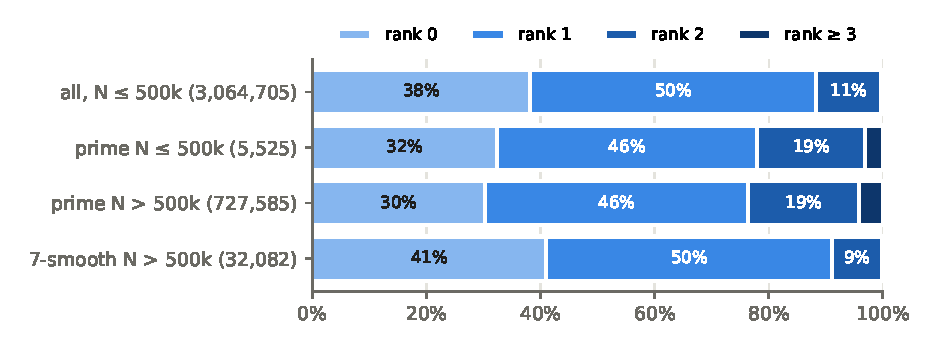
\includegraphics[width=\linewidth]{step01_regimes.pdf}
\caption{Rank mix by group, with the number of curves in each. Prime-conductor curves
have the same mix below and above $500{,}000$; the complete range below $500{,}000$ is
different because most of its conductors are composite.}
\label{fig:regimes}
\end{figure}

\paragraph{The rank mix drifts with the conductor.}
Even inside the complete range the mix is not stable (Figure~\ref{fig:drift}). Between the
first and last bins of $25{,}000$ conductors, the share of rank~2 rises from
\RankTwoFirstBin{} to \RankTwoLastBin{}, and rank~0 falls from \RankZeroFirstBin{} to
\RankZeroLastBin. Conjecturally, half of all curves have rank 0 and half rank 1, so this
excess of rank~2 is expected to fade at much larger conductors, too slowly to see here.
Bektemirov, Mazur, Stein and Watkins discuss this tension between tables and conjecture
(\emph{Average ranks of elliptic curves}, Bull.\ AMS, 2007). Two consequences for us:
the conductor alone carries information about the label, and any test on larger conductors
faces a different class balance, a \emph{label shift}, even before the features change.

\begin{figure}[ht]
\centering
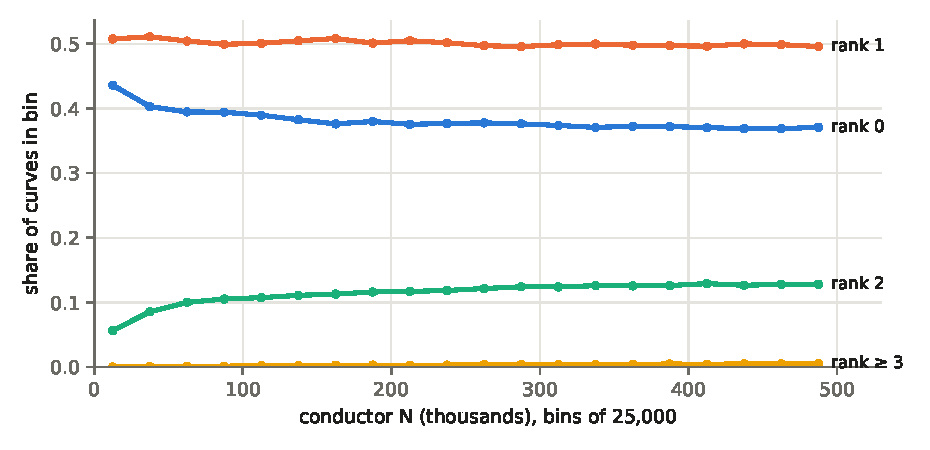
\includegraphics[width=\linewidth]{step01_rank_by_conductor.pdf}
\caption{Share of each rank among curves of conductor $N\le500{,}000$, in bins of
$25{,}000$.}
\label{fig:drift}
\end{figure}

\paragraph{What this means for Task~2.}
Task~2 keeps the \NTaskTwo{} curves of rank 0 or 2. Overall \PiTaskTwo{} of them have rank~2,
but that rate is \PiTaskTwoComplete{} in the complete range, \PiTaskTwoSmallPrime{} for
prime conductors below $500{,}000$, and \PiTaskTwoHighPrime{} for prime conductors above it.
A model trained on the complete range and tested on the large prime-conductor curves would
face both a different kind of conductor and a different base rate. So Section~3 will run two
tests: a clean one, prime conductors below $500{,}000$ against prime conductors above it, and
the harder one across the boundary.

\paragraph{A first look at leakage.}
The last column is the analytic order of $\Sha$. It exceeds $1$ for \ShaBigRankZero{} of
rank-0 curves but only \ShaBigRankTwo{} of rank-2 curves. The column is computed from the
BSD formula, which needs the rank and the leading coefficient. And empirically, as in
Delaunay's heuristics for $\Sha$, nontrivial $\Sha$ is much rarer on curves of higher rank. A model given this column would learn ``$\Sha>1$ means rank 0''
and look clever. It stays out of every feature set, as Section~0 promised.

\paragraph{What this step cannot tell us.}
The checks confirm that each row describes a real, minimal curve with the stated conductor.
They cannot confirm the ranks: those come from descents and $L$-function computations that we
are trusting, not redoing. Section~2 begins computing things we \emph{can} check ourselves:
the $a_p$, by counting points.

\paragraph{Exercises.}
\begin{exercise}\label{ex:isogeny-rank}
Let $\varphi:E\to E'$ be an isogeny over $\Q$. Show that $\rk E(\Q)=\rk E'(\Q)$. (Use the dual
isogeny $\hat\varphi$ with $\hat\varphi\circ\varphi=[\deg\varphi]$, and that $\ker\varphi$ is finite.)
\end{exercise}
\begin{exercise}\label{ex:isogeny-ap}
Show that isogenous curves have $\#E(\F_p)=\#E'(\F_p)$ for every good prime $p$, so their
$a_p$ agree. Then suppose we split curves (not classes) at random, 80\% to training. Using the
class sizes, estimate what fraction of test curves have an isogenous twin in training. Why is
that fraction an underestimate of the damage when the model is very flexible?
\end{exercise}
\begin{exercise}\label{ex:label-shift}
A model is calibrated on a population where rank~2 has base rate $\pi$, and then used on one
with base rate $\pi'$. Assume pure \emph{label shift}: the distribution of features given the
rank is the same in both. Show that the correct probability on the new population is
obtained by multiplying the predicted odds by $\frac{\pi'/(1-\pi')}{\pi/(1-\pi)}$. Evaluate the
factor for the complete range versus large prime conductors in Task~2.
\end{exercise}

\begin{interview}
\emph{``How did you validate the data?''} ``Ten checks, each with a test that corrupts a row
to prove it can fail. The strongest uses the fact that for a minimal model the bad primes are
exactly the primes of the discriminant, which catches typos, non-minimal models and wrong
conductors in one go. Then I asked where the data came from: everything above conductor
500{,}000 has prime or 7-smooth conductor, so the `generalize to larger conductors' test is
really a test on a different family. I compare like with like, prime conductors below
500{,}000 against prime conductors above it.''
\end{interview}

%=============================================================================
\appendix
\section*{Solutions to exercises}
\addcontentsline{toc}{section}{Solutions to exercises}
%=============================================================================

\paragraph{Exercise \ref{ex:parity}.}
The gamma factor is nonzero at $s=1$ ($\Gamma(1)=1$), so $\ord_{s=1}\Lambda=r_{\mathrm{an}}$ and
$\Lambda(E,s)=c\,(s-1)^{r}+O((s-1)^{r+1})$ with $c\neq0$ and $r=r_{\mathrm{an}}$. Substituting
$s\mapsto2-s$ gives $\Lambda(E,2-s)=c\,(1-s)^{r}+\dots=(-1)^{r}c\,(s-1)^{r}+\dots$. Comparing
leading coefficients in \eqref{eq:fe} gives $c=w(-1)^{r}c$, so $w=(-1)^{r}$.

\paragraph{Exercise \ref{ex:semistable}.}
With $w=-\prod_{p\mid N}w_p$ and $w_p=-a_p$ for every $p\mid N$,
$w=-\prod_{p\mid N}(-a_p)=-(-1)^{\omega(N)}\prod a_p=(-1)^{\omega(N)+1}\prod a_p$.
For \code{11.a}: $\omega=1$, $a_{11}=1$, so $w=+1$, consistent with rank $0$.
For \code{37.a}: $\omega=1$, $a_{37}=-1$, so $w=-1$, consistent with rank $1$.

\paragraph{Exercise \ref{ex:baseline}.}
A constant prediction of class~$1$ is right on a fraction $\pi$ of curves and class~$0$ on
$1-\pi$; take the larger. A constant probability $q$ has expected log-loss
$-\pi\log q-(1-\pi)\log(1-q)$, minimized at $q=\pi$ with value $H(\pi)$. When $\pi$ is small,
predicting ``rank $0$'' always scores $1-\pi$, close to $1$, while finding no rank-$2$ curve at
all. Log-loss rewards confidence that is justified, and PR-AUC measures how well the model
ranks the rare class, so both expose that predictor.

\paragraph{Exercise \ref{ex:isogeny-rank}.}
$\varphi$ restricts to a homomorphism $E(\Q)\to E'(\Q)$ with finite kernel, so
$\rk E(\Q)\le\rk E'(\Q)$. The dual isogeny $\hat\varphi:E'\to E$ is also defined over $\Q$ with
finite kernel, giving the reverse inequality.

\paragraph{Exercise \ref{ex:isogeny-ap}.}
For good $p$, $\varphi$ reduces to an isogeny $\tilde E\to\tilde E'$ over $\F_p$ that commutes
with Frobenius $\pi$. Then $\#\tilde E(\F_p)=\deg(1-\pi)$ on both sides, since $1-\pi$ has the
same characteristic polynomial on the Tate modules, which the isogeny identifies after
tensoring with $\Q_\ell$. With random curve-level splitting, a test curve in a class of size
$k$ has an untouched twin unless all $k-1$ others also went to test, so the fraction is
$\sum_k f_k\,(1-0.2^{k-1})$, where $f_k$ is the share of curves in classes of size $k$. It
underestimates the damage because a flexible model memorizes the exact $a_p$ vector, so one
twin is enough to recall the label.

\paragraph{Exercise \ref{ex:label-shift}.}
By Bayes, the posterior odds are the likelihood ratio $p(x\mid r=2)/p(x\mid r=0)$ times the
prior odds. Under label shift the likelihood ratio is unchanged, so the new odds are the old
odds divided by $\pi/(1-\pi)$ and multiplied by $\pi'/(1-\pi')$. With the numbers from this
section, the factor is about $(0.391/0.609)/(0.229/0.771)\approx2.2$: the model should more than
double its odds of rank~2 on the large prime-conductor curves.

\end{document}
